
 

The wealth and diversity of experimental data in the life sciences has been a strong catalyst in the increasingly ubiquitous nature of classification methods in computational biology. Over the past couple of decades the scope and sophistication of these methods has significantly increased; growing from relatively simple procedures based on na\"ive Bayes or logistic regression  into fully fledged Bayesian and structured-output learning methods. One of the important factors leading to the increased adoption of modern classification models in computational biology is their ability to not only integrate various types of data, be it sequence, structure, graphs or text; but also their robustness when dealing with data of varying degrees of quality. Methods attuned to producing quality predictions on a particular type of biological data; or that can facilitate the integration of data from disparate sources, have been quickly adopted by the community.

Among the various classification strategies, kernel-based methods have recently become prominent \citep{shawe2004kernel}. In general, kernels can be described as similarity functions that operate on pairs of objects and maintain certain mathematical properties. One important characteristic of kernel-based methods that distinguishes them from traditional machine learning approaches is individual objects need not be explicitly represented in a vector, or feature, space $\mathcal{F}$ (even if they often are); an inner product space is obtained through the similarities generated by applying the kernel function to pairs of objects, 

\[
k(\mathbf{x}_{1},\mathbf{x}_{2}) = \langle \phi (\mathbf{x}_{1}), \phi (\mathbf{x}_{2}) \rangle, 
\]
where $\mathnormal{\phi} (\mathbf{x})$ represents the embedding of object $\mathbf{x}$ in $\mathcal{F}$.  Through the kernel function, $k(\mathbf{x}_{1},\mathbf{x}_{2})$, objects are implicitly embedded in $\mathcal{F}$,  where linear relations (i.e. an optimal separating hyperplane between two classes) are searched for. Kernel approaches are therefore capable of operating on a broad class of input spaces by effectively mapping objects into unknown and potentially infinite dimensional feature spaces. When coupled with support vector machines, they also guarantee that a globally optimal solution to the optimization problem can be found. Although most kernel-based approaches are in practice formed by vectorizing input objects; not fully exploiting their theoretical potential, they still enable a practitioner to incorporate domain knowledge into modeling the relationship between objects, rather than simply encoding properties of the objects into a potentially high dimension vector space and providing them to a standard classifier.


Kernel approaches have been widely used in computational biology \citep{schoolkopf2004kernel}; being applied in a range of contexts such as the prediction of remote homology \citep{Leslie2002}, protein structure \citep{qiu2007structural} and function \citep{Vert2002,Vacic2010,Xin2011}, protein-protein interactions \citep{BenHur2005}, disease-gene prioritization \citep{DeBie2007}, the activity of chemical compounds \citep{ralaivola2005graph}, etc. An excellent summary and history of early approaches has been provided by \citet{noble2004kernel}. Most of these approaches have been used to predict properties of proteins, either in terms of entire sequences or individual residues. For example, the most influential kernel methods were proposed to provide inferences regarding remote homology and function from amino acid sequences \citep{Leslie2002,jaakkola1999using,jaakkola2000discriminative,kuang2004profile}. Graph kernels, first introduced by \cite{kondor2002diffusion}, have gained significant attention in computational biology due to the potential for modeling a variety of data types through graphs \citep{borgwardt2005protein}. A number of approaches also considered integration of kernels built on different types of data, including scientific text \citep{Sokolov2010}. 


For the purposes of this work, we focus our investigation on the viability of kernel approaches in terms of type of data used when forming a kernel representation of proteins. We develop novel methodology for the non-alignment kernel-based supervised classification of protein sequences and structures into distinct categories. In contrast to most previously implemented kernel approaches, we represent a protein�s sequence or structure, if available, as a set of time series properties such as hydrophobicity profile or predicted propensity of secondary structure types, calculated by considering an individual amino acid and its flanking regions. 

An important problem in calculating the similarity between differing length real-valued vectors is providing a fixed-length representation to be used as input for a given prediction method. To do this, we use the ideas of vector quantization. Vector quantization (VQ) was initially developed as a lossy method for compressing signals \citep{Linde1980algorithm}. We evaluated methods on two distinct and relevant problems: ($i$) the classification of protein structures into structural classes and ($ii$) the prediction of protein function from amino acid sequence.


%% Figure
%%%%%%%%%%%%%%%%%%%%%%
%%%%%%%%%%%%%%%%%%%%%%
%%%%%%%%%%%%%%%%%%%%%%
%%%%%%%%%%%%%%%%%%%%%%
\begin{figure*}[ht!]
\begin{centering}

	\begin{subfigure}[b]{0.40\textwidth}
                \centering
	     	
\includegraphics[width=\textwidth]{Figures/VQ/TimeSeries/Kappa}
		\caption{$\kappa$ angles}
		\label{fig:kappaTS}
        \end{subfigure}
	\quad
	\begin{subfigure}[b]{0.40\textwidth}
                \centering
	     	
\includegraphics[width=\textwidth]{Figures/VQ/TimeSeries/Alpha}
		\caption{$\alpha$ angles}
		\label{fig:alphaTS}
      \end{subfigure}


	\begin{subfigure}[b]{0.40\textwidth}
                \centering
	     	
\includegraphics[width=\textwidth]{Figures/VQ/TimeSeries/Phi}
		\caption{$\phi$ angles}
		\label{fig:phiTS}
	\end{subfigure}		
	\quad
	\begin{subfigure}[b]{0.40\textwidth}
                \centering
	     	
\includegraphics[width=\textwidth]{Figures/VQ/TimeSeries/Psi}
		\caption{$\psi$ angles}
		\label{fig:psiTS}
      \end{subfigure}	


	\begin{subfigure}[b]{0.40\textwidth}
                \centering
	     	
\includegraphics[width=\textwidth]{Figures/VQ/TimeSeries/Helix}
		\caption{Predicted helix}
		\label{fig:helixTS}
      \end{subfigure}
	\quad
	\begin{subfigure}[b]{0.40\textwidth}
                \centering
	     	
\includegraphics[width=\textwidth]{Figures/VQ/TimeSeries/SolAcc}
		\caption{Solvent accessibility}
		\label{fig:solaccTS}
      \end{subfigure}


%	\begin{subfigure}[b]{0.65\columnwidth}
%                \centering
%	     	
\includegraphics[width=0.65\columnwidth]{Figures/VQ/TimeSeries/VSL2B}
%		\caption{Predicted disorder}
%		\label{fig:disorderTS}
%      \end{subfigure}

\caption[Time Series Representation of Protein Properties]{Time series representation of various protein properties for the 73 amino acid long DNA helicase RuvA subunit \bf{d1ixra1}.}
\end{centering}
\label{fig:TimeSeries}
 \end{figure*}

%%%%%%%%%%%%%%%%%%%%%%
%%%%%%%%%%%%%%%%%%%%%%

%%%%%%%%%%%%%%%%%%%%%%
%%%%%%%%%%%%%%%%%%%%%%
\section{Problem formulation}
%%%%%%%%%%%%%%%%%%%%%%
%%%%%%%%%%%%%%%%%%%%%%


In this chapter we represent a protein as a set of time series properties such as hydrophobicity profiles, predictions of intrinsically disordered regions, or dihedral angle values if its structure is available (\Cref{fig:TimeSeries}). One way to augment the differing length time series signals for each sequence into fixed length features to be used as input for a given prediction method is to apply a vector quantization (VQ) kernel. The basic idea behind this method (outlined in Figure \ref{fig:VQ_schematic}) is to first break each signal up into overlapping fixed $n-$length segments (Figure \ref{fig:VQ_schematic}a). These small segments are then clustered in $n$-dimensional space, generating a set of $m$ centroids representing each cluster (Figure \ref{fig:VQ_schematic}b). We chose to use k-means clustering as opposed to simply creating a lattice in $n$-dimensional space, as done by \citet{Tuytelaars2007}, because sampled property vectors do not fill the space evenly, but instead cluster around evolutionarily conserved or sterically preferred ``regions". After clustering, each segment can then be represented by which cluster it belongs to, and counts (or relative frequencies) that each subsegment for a property belongs to a cluster can be used to represent a sequence (Figure \ref{fig:VQ_schematic}c). 

%%%%%%%%%%%%%%%%%%%%%
%%%%%%%%%%%%%%%%%%%%%
\begin{figure*}[h!]
\begin{centering}
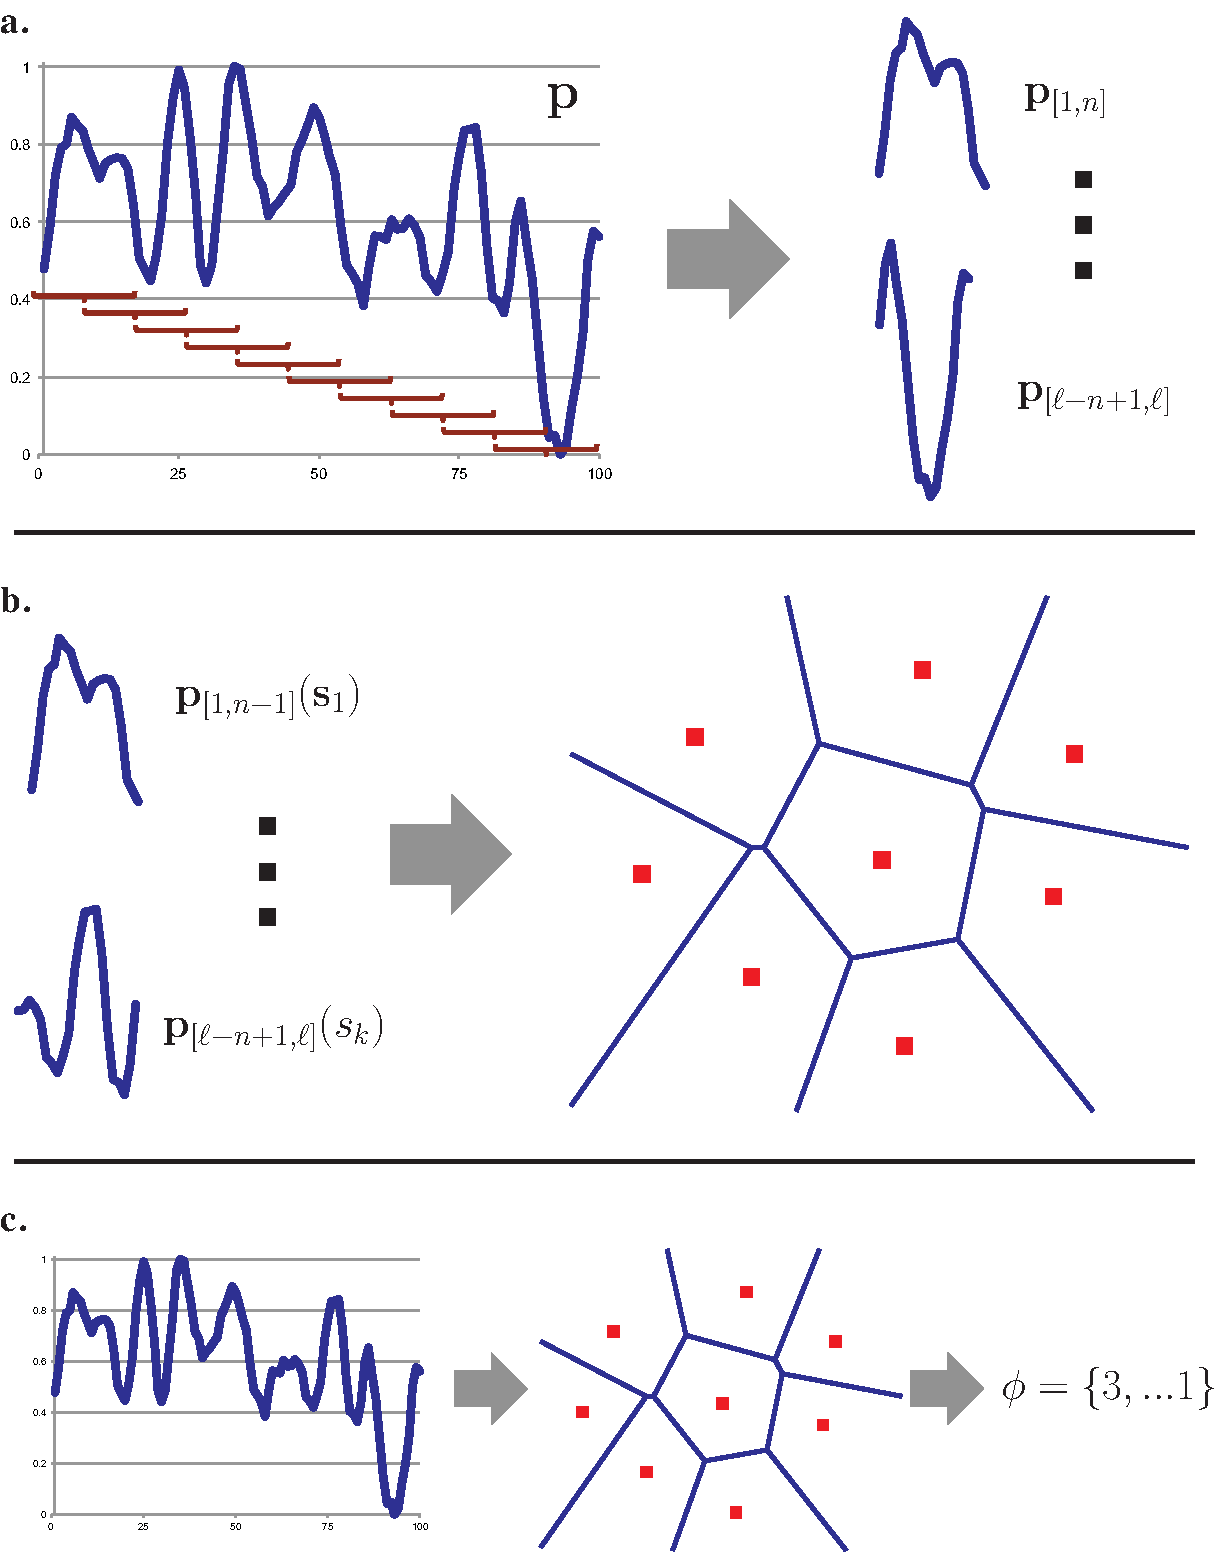
\includegraphics[width=.50\linewidth]{Figures/vq/VQ_FIG}
\par\end{centering}
\caption[A schematic representation of using VQ to encode a sequence represented as a property vector]{A schematic representation of using VQ to encode a sequence represented as a property vector. In \ref{fig:VQ_schematic}(a) an individual property vector is broken up into $n$ length subsamples. In this example the amount of overlap is $\frac{n}{2}$, although differing values can be used, including randomly choosing samples in instances with a large number of sequences. \ref{fig:VQ_schematic}(b), subsampled vectors from a database of sequences are used to create a clustering in $n$-dimensional space, with centroids represented as red squares. Finally, in \ref{fig:VQ_schematic}(c) an original property vector is encoded using the derived set of centroids by counting the number of sub-vectors which are the closest to each centroid. In this case, sub sampled vectors are usually shifted by a single amino acid.}
\label{fig:VQ_schematic}
\end{figure*}
%%%%%%%%%%%%%%%%%%%%%
%%%%%%%%%%%%%%%%%%%%%
